\documentclass[aspectratio=169]{beamer}
\beamertemplatenavigationsymbolsempty
\usepackage[utf8]{inputenc}
\usepackage[T1]{fontenc}
\usepackage{lmodern}
\usepackage{bm}
\usepackage{amsmath,amssymb}
\usepackage{booktabs}
\usepackage{tikz}
\usetikzlibrary{positioning,arrows.meta,shapes.geometric,calc}
\usepackage{graphicx}
\usepackage{tabularx}
\usepackage{array}
\usepackage{xcolor}
\usepackage{colortbl}
\usepackage{pifont}
\usepackage{makecell}
\usepackage{adjustbox}

% Weekly update, October 2, 2026: how the detection mechanism changed and how
% the earlier results leaked the fault family.  Style follows the 16:9
% Madrid/beaver weekly template.  Sources are listed on the last slide.
% Build: pdflatex -interaction=nonstopmode -halt-on-error weekly_update_20261002.tex

% ====== Macros ======
\newcommand{\cmark}{\textcolor{green!60!black}{\ding{51}}}
\newcommand{\xmark}{\textcolor{red!70!black}{\ding{55}}}
\newcommand{\good}[1]{\textcolor{green!50!black}{\textbf{#1}}}
\newcommand{\bad}[1]{\textcolor{red!70!black}{\textbf{#1}}}
\newcommand{\warn}[1]{\textcolor{orange!80!black}{\textbf{#1}}}
\newcommand{\code}[1]{\texttt{\detokenize{#1}}}
\newcommand{\tightvspace}{\vspace{0.35em}}
\newcommand{\reportsource}[1]{{\vskip 0.4em\tiny\textcolor{gray!80!black}{\textbf{Source:} #1}\par}}
% Used by the template's slides but not defined in its preamble.
\newcommand{\scope}[1]{{\small\textit{#1}}\par\vspace{0.4em}}

\newcolumntype{Y}{>{\raggedright\arraybackslash}X}
\newcolumntype{P}[1]{>{\raggedright\arraybackslash}p{#1}}
\newcolumntype{L}[1]{>{\raggedright\arraybackslash}p{#1}}

\usetheme{Madrid}
\usecolortheme{beaver}
\setbeamertemplate{caption}[numbered]
\setlength{\tabcolsep}{4pt}
\renewcommand{\arraystretch}{1.12}
% Beamer's \appendix puts \translate into the PDF bookmarks.
\pdfstringdefDisableCommands{\def\translate#1{#1}}

\tikzset{
  stage/.style={draw=gray!65, rounded corners=2pt, fill=gray!7, align=center,
    inner sep=3pt, minimum height=0.8cm},
  gate/.style={stage, fill=orange!14, draw=orange!60!black},
  phys/.style={stage, fill=blue!7, draw=blue!45!black},
  leak/.style={stage, fill=red!8, draw=red!50!black},
  outc/.style={stage, fill=green!8, draw=green!40!black},
  arr/.style={-{Stealth[length=1.8mm]}, thick, gray!70!black},
  lab/.style={font=\tiny\itshape, fill=white, inner sep=1pt},
}

\title[Power System LLM]{Weekly Report}
\subtitle{How Detection Changed and How Earlier Results Leaked}
\author{Yifei Xu}
\institute{New York University}
\date{October 2, 2026}

\begin{document}
\maketitle

% 2
\begin{frame}{This Week's Changes}
  \begin{itemize}
    \setlength\itemsep{0.7em}
    \item \textbf{Leak found:} in the earlier runs, \emph{which data existed} told the agent the fault family. Detection itself was never tested.
    \item \textbf{New detection:} balanced SCADA, WLS and a balanced hypothesis screen. Auxiliary data opens only on a balanced suspicion, and every root carries it.
    \item \textbf{Expert under the new contract:} \textbf{159/160} development roots, no false commit.
    \item \textbf{LLM pipeline:} rerun from scratch with the new teacher. First honest student score: \textbf{R1 158/160} (BC0 152, expert 160). Round 2 is running.
    \item \textbf{Screen cost:} about 1\,s per alarm. A gradient-boosted model on the WLS alone matches the request decision but not the HIF line; cheaper physics tests come first.
  \end{itemize}
\end{frame}

% 3
\begin{frame}{Earlier Scores and What They Assumed}
  \small
  \renewcommand{\arraystretch}{1.25}
  \begin{tabularx}{\textwidth}{L{1.9cm}L{2.5cm}rrY}
    \toprule
    Run & Evidence contract & Expert & Student & What the agent was given \\
    \midrule
    Sep 21--22 & auxiliary-assisted & 158/160 & R2 157/160 & HIF relay flag at reset; all auxiliary data always available \\
    Sep 24--27 & WLS-gated & 158/160 & R2 157/160 & no flag, but phasors and spectra existed only on their own family's roots \\
    Sep 22 check & SCADA-only & $\le$104/160 & -- & no auxiliary data at all \\
    \bottomrule
  \end{tabularx}
  \par\vspace{0.8em}
  \begin{itemize}
    \setlength\itemsep{0.4em}
    \item Neither 157/160 measures detection from balanced evidence.
    \item SCADA-only is the opposite extreme: the 56 HIF, meter+HIF, unbalance and harmonic roots are unreachable.
  \end{itemize}
  \reportsource{S1, S6, S8. Sep 21--22 scores use the revised runtime and audit of Sep 22.}
\end{frame}

% 4
\begin{frame}{Leak 1: The Request Answered the Family Question}
  \scope{WLS-gated contract, September 23--27}
  \begin{center}
  \begin{adjustbox}{max width=\textwidth}
  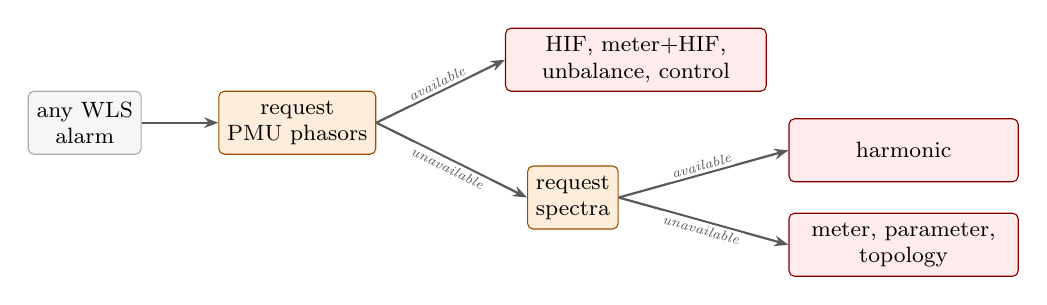
\begin{tikzpicture}[font=\footnotesize]
    \node[stage] (alarm) at (0,0) {any WLS\\alarm};
    \node[gate] (ph) at (2.7,0) {request\\PMU phasors};
    \node[leak, text width=3.1cm] (wave) at (7.0,0.8) {HIF, meter+HIF,\\unbalance, control};
    \node[gate] (sp) at (6.2,-0.95) {request\\spectra};
    \node[leak, text width=2.7cm] (harm) at (10.4,-0.35) {harmonic};
    \node[leak, text width=2.7cm] (bal) at (10.4,-1.55) {meter, parameter,\\topology};
    \draw[arr] (alarm) -- (ph);
    \draw[arr] (ph.east) -- node[lab, above, sloped] {available} (wave.west);
    \draw[arr] (ph.east) -- node[lab, below, sloped] {unavailable} (sp.west);
    \draw[arr] (sp.east) -- node[lab, above, sloped] {available} (harm.west);
    \draw[arr] (sp.east) -- node[lab, below, sloped] {unavailable} (bal.west);
  \end{tikzpicture}
  \end{adjustbox}
  \end{center}
  \small
  \begin{itemize}
    \setlength\itemsep{0.2em}
    \item Routing rule: after \emph{any} WLS alarm, request phasors; if unavailable, request spectra.
    \item Each stream existed only where the ground truth needed it, so one or two answers classified the root.
    \item HIF, unbalance and harmonic were \textbf{16/16 for expert, BC0, R1 and R2}, with the family known before any balanced evidence was weighed.
  \end{itemize}
  \reportsource{S1 (``Availability-based cues''), S6.}
\end{frame}

% 5
\begin{frame}{Other Leaks: Family Cues in the Data and Tools}
  \footnotesize
  \renewcommand{\arraystretch}{1.12}
  \begin{tabularx}{\textwidth}{L{3.5cm}YL{2.6cm}}
    \toprule
    Cue & What it gave away & Status \\
    \midrule
    Bus-9 capacitor counted twice in OpenDSS exports & every legacy HIF and unbalance row alarmed through bus-9 $Q$ (median $J=246$, limit 130); without it only 75/220 unbalance rows alarm & fixed Sep 19--21 \\
    Generator kW write reset its reactive limits & bus-8 $Q_{\rm inj}\approx0$ on every HIF row, 0.14--0.24 pu elsewhere & fixed Sep 23 \\
    OpenDSS families at default dispatch & bus-3 $P$ and bus-8 $V$ separated them from the OPF families & fixed Sep 23 \\
    HIF replay without voltage regulation & GNN pure-HIF recall 64.1\% $\to$ 46.9\% once regulation is emulated & GNN blocked in strict profiles \\
    HIF estimators replayed the simulator operating point & truth inside the diagnosis; scan windows only on HIF roots & removed Sep 27 \\
    \bottomrule
  \end{tabularx}
  \par\vspace{0.5em}
  \small The capacitor made the WLS alarm itself an artifact. The bus-8 and dispatch cues let a learned model read the family from SCADA values.
  \reportsource{S1, S9, S10, S11.}
\end{frame}

% 6
\begin{frame}{How the Detection Contract Changed}
  \footnotesize
  \renewcommand{\arraystretch}{1.22}
  \begin{tabularx}{\textwidth}{L{1.55cm}L{2.55cm}L{2.75cm}YL{2.0cm}}
    \toprule
    Date & Contract & Detection & Auxiliary data opens on & Carried by \\
    \midrule
    to Sep 21 & auxiliary-assisted & HIF relay flag; WLS & always & own family \\
    Sep 22 & SCADA-only & WLS alarm & never & -- \\
    Sep 23 & WLS-gated & WLS alarm & any alarm & own family \bad{(leak)} \\
    Sep 27 & suspicion-gated & WLS + HIF screen & HIF suspicion & \good{every root} \\
    Sep 30 & suspicion-gated v2 & WLS + hypothesis screen & HIF, voltage-meter or unexplained; spectra after balanced phasors & \good{every root} \\
    Oct 1 & + ledger and ranker & same & same; the ranker may defer one request & \good{every root} \\
    \bottomrule
  \end{tabularx}
  \par\vspace{0.7em}
  \small Alarm test throughout:
  \[J=e^\mathsf{T}R^{-1}e\geq\chi^2_{\nu,0.99}\quad\text{or}\quad\max_i|r_i^N|\geq4.\]
  \reportsource{S1, S2, S3.}
\end{frame}

% 7
\begin{frame}{The New Detection Pipeline}
  \begin{center}
  \begin{adjustbox}{max width=\textwidth}
  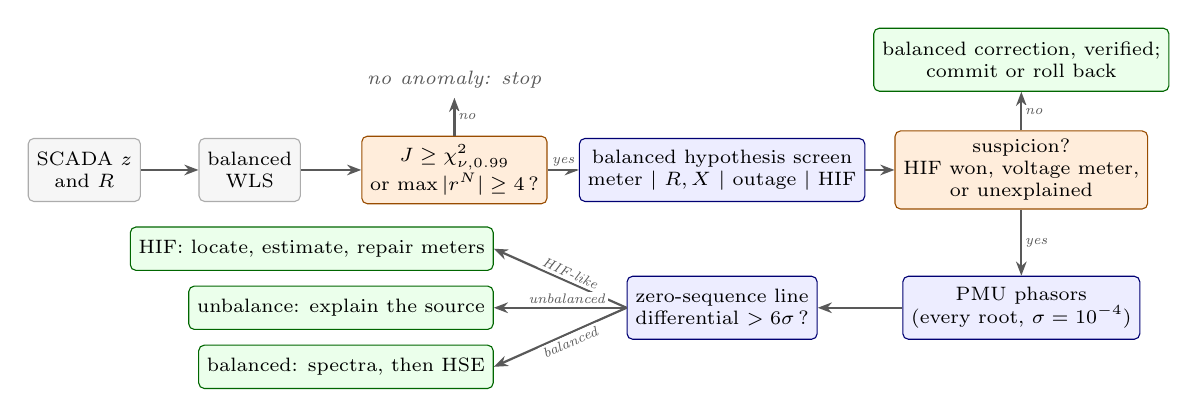
\begin{tikzpicture}[font=\scriptsize]
    \node[stage] (z) at (0,0) {SCADA $z$\\and $R$};
    \node[stage] (wls) at (2.1,0) {balanced\\WLS};
    \node[gate] (alarm) at (4.7,0) {$J\geq\chi^2_{\nu,0.99}$\\or $\max|r^N|\geq4$\,?};
    \node[phys] (screen) at (8.1,0) {balanced hypothesis screen\\meter $\mid$ $R,X$ $\mid$ outage $\mid$ HIF};
    \node[gate] (sus) at (11.9,0) {suspicion?\\HIF won, voltage meter,\\or unexplained};
    \node[font=\scriptsize\itshape, text=gray!70!black] (ok) at (4.7,1.15) {no anomaly: stop};
    \node[outc] (fix) at (11.9,1.4) {balanced correction, verified;\\commit or roll back};
    \node[phys] (pmu) at (11.9,-1.75) {PMU phasors\\(every root, $\sigma=10^{-4}$)};
    \node[phys] (zs) at (8.1,-1.75) {zero-sequence line\\differential $>6\sigma$\,?};
    \node[outc, minimum height=0.55cm, anchor=east] (hif) at (5.2,-1.0) {HIF: locate, estimate, repair meters};
    \node[outc, minimum height=0.55cm, anchor=east] (unb) at (5.2,-1.75) {unbalance: explain the source};
    \node[outc, minimum height=0.55cm, anchor=east] (har) at (5.2,-2.5) {balanced: spectra, then HSE};
    \draw[arr] (z) -- (wls);
    \draw[arr] (wls) -- (alarm);
    \draw[arr] (alarm) -- node[lab, above] {yes} (screen);
    \draw[arr] (alarm) -- node[lab, right] {no} (ok);
    \draw[arr] (screen) -- (sus);
    \draw[arr] (sus) -- node[lab, right] {no} (fix);
    \draw[arr] (sus) -- node[lab, right] {yes} (pmu);
    \draw[arr] (pmu) -- (zs);
    \draw[arr] (zs.west) -- node[lab, above, sloped, pos=0.45] {HIF-like} (hif.east);
    \draw[arr] (zs.west) -- node[lab, above, pos=0.45] {unbalanced} (unb.east);
    \draw[arr] (zs.west) -- node[lab, below, sloped, pos=0.45] {balanced} (har.east);
  \end{tikzpicture}
  \end{adjustbox}
  \end{center}
  \small
  \begin{itemize}
    \setlength\itemsep{0.2em}
    \item Everything before the phasor box uses only SCADA, its covariance and the balanced model.
    \item A balanced correction that verification rejects also opens the phasors.
  \end{itemize}
  \reportsource{S2, S3, S11.}
\end{frame}

% 8
\begin{frame}{Balanced Hypothesis Screen}
  \small
  After a WLS alarm, refit the operator's balanced model under competing single causes:
  \begin{center}
    \renewcommand{\arraystretch}{1.08}
    \begin{tabular}{lll}
      \toprule
      Class & Refit & Free parameters \\
      \midrule
      Meter & one of the six largest residual channels set aside & its bias \\
      Parameter & one branch's $R$, $X$, or both, inside a plausible box & 1 or 2 \\
      Topology & one branch switched out, never islanding a bus & -- \\
      HIF & line split at $\alpha$, shunt $G\geq0$ at a new zero-injection bus & $G$ \\
      \bottomrule
    \end{tabular}
  \end{center}
  \vspace{-0.3em}
  \[s_c=J_0-J_c-\bigl(13.5\,n_{\rm cont}+0.25\ln n_{\rm cand}\bigr)\]
  \vspace{-0.6em}
  \begin{itemize}
    \setlength\itemsep{0.2em}
    \item Apply the winner and repeat, up to three comparisons, until the alarm clears or HIF wins.
    \item Outputs: accepted sequence (e.g.\ \code{parameter>meter}), HIF line, voltage channels set aside, \emph{unexplained}.
  \end{itemize}
  \reportsource{S3, S11 (\texttt{hif\_screen.py}; penalties tuned on the Sep 26 design half).}
\end{frame}

% 9
\begin{frame}{What Opens Auxiliary Data Now}
  \small
  \renewcommand{\arraystretch}{1.25}
  \begin{tabularx}{\textwidth}{L{3.4cm}Y}
    \toprule
    Request & Admitted only when \\
    \midrule
    PMU phasors, phasor test & HIF won; a phase-A voltage channel was set aside; the alarm stayed unexplained; or verification rejected the screen's explanation \\
    HIF estimator & screen HIF, or a zero-sequence differential above $6\sigma$ \\
    Spectra, HSE & phasors on this state came back balanced \\
    Voltage-meter edit & waits for phasors while a phasor suspicion stands \\
    \bottomrule
  \end{tabularx}
  \par\vspace{0.7em}
  \begin{itemize}
    \setlength\itemsep{0.35em}
    \item Every root carries true-state phasors and noise-only spectra, so \textbf{no request answers by availability}.
    \item The phasor test uses each line's terminal differential: a fault to ground leaves a zero-sequence part; a balanced model error leaves none.
  \end{itemize}
  \reportsource{S2, S3, S11 (\texttt{suspicion\_gated.py}, \texttt{evidence\_profile.py}).}
\end{frame}

% 10
\begin{frame}{Same Root Types, Old and New Traces}
  \small
  \renewcommand{\arraystretch}{1.35}
  \begin{tabularx}{\textwidth}{L{2.1cm}YY}
    \toprule
    Root & WLS-gated (Sep 23) & Suspicion-gated (now) \\
    \midrule
    Unbalance & alarm $\to$ phasors \bad{available} $\to$ phasor test $\to$ explain & alarm $\to$ screen picks a voltage meter $\to$ phasors $\to$ phasor test finds the unbalance $\to$ explain \\
    Harmonic & alarm $\to$ phasors \bad{unavailable} $\to$ spectra \bad{available} $\to$ HSE & alarm $\to$ screen: unexplained $\to$ phasors come back balanced $\to$ spectra $\to$ HSE \\
    Bad power meter & alarm $\to$ phasors \bad{unavailable} $\to$ spectra \bad{unavailable} $\to$ meter route & alarm $\to$ screen picks the meter $\to$ meter route, no request \\
    \bottomrule
  \end{tabularx}
  \par\vspace{0.9em}
  The old answers did the classification. The new answers are measurements the agent has to interpret, and a request needs a balanced reason.
  \reportsource{S1, S3 (expert traces under both contracts).}
\end{frame}

% 11
\begin{frame}{What Balanced Evidence Can Separate}
  \scope{Screen on the step-1 dataset: 2,148 alarmed fault roots and 69 alarmed healthy windows}
  \footnotesize
  \renewcommand{\arraystretch}{1.06}
  \begin{center}
  \begin{tabular}{lrrrrr}
    \toprule
    Family & Alarmed & HIF flag & Voltage-meter pick & Unexplained & Phasor rule fires \\
    \midrule
    HIF & 131 & \good{130} & 0 & 0 & 130 \\
    Meter + HIF & 131 & \good{128} & 0 & 0 & 128 \\
    Unbalance & 162 & 0 & 160 & 77 & 161 \\
    Harmonic & 250 & 0 & 248 & 208 & 249 \\
    Single meter & 250 & 0 & 33 & 0 & 33 \\
    Multiple meters & 224 & 0 & 28 & 113 & 126 \\
    Topology & 250 & 0 & 11 & 55 & 55 \\
    Parameter, mixed balanced & 750 & 0 & 2 & 0 & 2 \\
    Healthy windows & 69 & 1 & 10 & 2 & 13 \\
    \bottomrule
  \end{tabular}
  \end{center}
  \small The HIF flag fires on 258 of 262 HIF roots and on no other fault root. Unbalance and harmonic look like a bad voltage meter, so phasors decide. The rule fires on 216 of the 1,474 balanced-family roots.
  \reportsource{S3 (screen v3, as shipped).}
\end{frame}

% 12
\begin{frame}{Expert Results Under Each Contract}
  \scope{Rule-based expert, 160 development roots, deployment-mode verifier, 40 actions}
  \begin{center}
    \small
    \renewcommand{\arraystretch}{1.18}
    \begin{tabular}{llr}
      \toprule
      Contract & Note & Expert \\
      \midrule
      WLS-gated (Sep 24) & family known from availability & \bad{158/160} \\
      SCADA-only & waveform families unreachable & $\le$104/160 \\
      HIF-only gate (Sep 27) & unbalance and harmonic uncredited & $\le$128/160 \\
      Screen v2 + rule v3 & baseline expert & \good{159/160} \\
      Screen v2 + rule v3 & hypothesis-ledger expert & \good{159/160} \\
      Same, + learned ranker & HPC teacher, cell's own draw & \good{160/160} \\
      \bottomrule
    \end{tabular}
  \end{center}
  \begin{itemize}
    \setlength\itemsep{0.25em}
    \item Fresh check: \textbf{48/48} roots over all 12 families; unbalance in 4 steps, harmonic in 6.
    \item Ledger: 8.1 vs 8.8 steps per episode, 8 vs 15 rejected candidates; no false commit in either.
    \item The one miss is an adjacent-line parameter root that both rankings get wrong.
  \end{itemize}
  \reportsource{S2, S3, S4, S6. The Sep 24 row is that cell's own draw; the rule-v3 rows share a fresh draw with the same family plan. Ceilings count unreachable families.}
\end{frame}

% 13
\begin{frame}{Fewer Unneeded Acquisitions: Learned Ordering}
  \scope{Gradient-boosted model on 73 policy-visible features; test split, 463 alarmed roots}
  \begin{center}
    \small
    \renewcommand{\arraystretch}{1.22}
    \begin{tabular}{lrr}
      \toprule
      & Physics rule & Learned score \\
      \midrule
      Recall, roots that need auxiliary data & 98.5\% & 99.2\% \\
      Acquisitions on roots that need none & 12.0\% & \good{2.1\%} \\
      Same-sign flow-meter pairs flagged as HIF & 37.5\% & \good{0\%} \\
      \bottomrule
    \end{tabular}
  \end{center}
  \begin{itemize}
    \setlength\itemsep{0.3em}
    \item The physics rule stays the gate. The score only lets the expert try its leading balanced hypothesis once before an admitted request.
    \item Paired on 208 roots: \textbf{63 vs 72} phasor requests at equal success; no root that needs phasors was deferred.
    \item IEEE-57 operating points do not transfer; the model refuses another network.
  \end{itemize}
  \reportsource{S5.}
\end{frame}

% 14
\begin{frame}{What the Screen Costs}
  \scope{IEEE-14; opening WLS of the 144 alarmed development roots; one core}
  \begin{columns}[T]
    \begin{column}{0.53\textwidth}
      \centering\footnotesize
      \renewcommand{\arraystretch}{1.18}
      \begin{tabular}{llr}
        \toprule
        Class & Candidates per round & Refits \\
        \midrule
        Meter & six largest residuals & 6 \\
        Parameter & 20 branches $\times$ $R$, $X$, both & 60 \\
        Outage & branches that island no bus & 19 \\
        HIF & 16 lines $\times$ 9 positions & 144 \\
        \midrule
        One round & & \textbf{229} \\
        \bottomrule
      \end{tabular}
    \end{column}
    \begin{column}{0.43\textwidth}
      \centering\footnotesize
      \renewcommand{\arraystretch}{1.18}
      \begin{tabular}{lrr}
        \toprule
        & Median & Max \\
        \midrule
        WLS solve alone & 0.05 s & 0.43 s \\
        Screen & \warn{1.1 s} & 3.0 s \\
        Refits per screen & 448 & 692 \\
        \bottomrule
      \end{tabular}
    \end{column}
  \end{columns}
  \vspace{0.3em}
  \footnotesize
  \begin{itemize}
    \setlength\itemsep{0.2em}
    \item Every refit is a full constrained WLS of the modified model, started from the alarmed solution; cached per state.
    \item 64 screens stop after one round, 37 after two, 43 after three; with two meters set aside a round costs 85 refits.
    \item Collection takes about 33 s per root, so on IEEE-14 the screen is a few seconds; refits grow with the branch count.
  \end{itemize}
  \reportsource{S12 (commit a76f704), S11.}
\end{frame}

% 15
\begin{frame}{Can a Gradient-Boosted Model Replace the Screen?}
  \scope{Step-4 dataset and splits; 463 alarmed test roots, 130 needing phasors or spectra, 50 with an HIF}
  \begin{center}
    \footnotesize
    \renewcommand{\arraystretch}{1.15}
    \begin{tabular}{lrrrr}
      \toprule
      & \multicolumn{2}{c}{Request gate} & \multicolumn{2}{c}{HIF flag} \\
      \cmidrule(lr){2-3}\cmidrule(lr){4-5}
      Decision from & Recall & Unneeded requests & Recall & False flags \\
      \midrule
      Physics rule and screen & 98.5\% & 12.0\% & 98\% & 1.5\% \\
      Gradient-boosted, alarmed WLS only & 98.5\% & 10.5\% & \bad{78\%} & 0.5\% \\
      Gradient-boosted, plus screen outputs & 96.9\% & \good{1.2\%} & 98\% & 1.7\% \\
      \bottomrule
    \end{tabular}
  \end{center}
  \footnotesize
  \begin{itemize}
    \setlength\itemsep{0.25em}
    \item With no refit, a model on residuals, multipliers and flow pairs matches the rule on \emph{whether} to request phasors.
    \item It misses the HIF line: at the screen's false-flag level it flags 39 of 50 HIF roots, against 49.
    \item The screen adds the HIF line and the ordered hypotheses; a model on its outputs cuts unneeded requests to 1.2\%.
    \item A learned-only gate needs retraining per network and can pick up simulator artifacts that name the family.
  \end{itemize}
  \reportsource{S12, S5. 45 single-solve features vs.\ the study's 94; thresholds from the calibration split. Slide 13: deployed 73-feature model.}
\end{frame}

% 16
\begin{frame}{Suggested Fixes}
  \footnotesize
  \renewcommand{\arraystretch}{1.06}
  \begin{tabularx}{\textwidth}{L{2.7cm}YL{2.5cm}L{2.2cm}}
    \toprule
    Fix & How & Saves & Status \\
    \midrule
    1.\ Linearized tests, refit a shortlist & Residuals score meters and Lagrange multipliers score branches, both from the alarmed WLS; an injection test scores HIF positions; refit the top one or two per class & most of the 229 refits per round, about tenfold & measure agreement with the full screen \\
    2.\ Two-stage gate & Screen-free model on every alarm; full screen only when it is uncertain or predicts phasors & the screen on confident balanced roots & to evaluate \\
    3.\ Parallel refits & Candidates are independent; about 16 cores per GPU on the cluster & wall time & engineering \\
    4.\ Spectra before a voltage-meter edit & When phasors come back balanced on a voltage-meter suspicion, request spectra first & 16 of the 26 extra actions below & next teacher \\
    \bottomrule
  \end{tabularx}
  \par\vspace{0.3em}
  \begin{itemize}
    \setlength\itemsep{0.2em}
    \item Expert today: 1,270 actions on 160 development roots against a shortest 1,244; 4 rollbacks, all on two harmonic roots.
    \item Order: fix 1 first, as it keeps the physics decisions and works on any network; fix 2 if larger networks stay slow.
  \end{itemize}
  \reportsource{S12 (teacher's own paths at commit a76f704).}
\end{frame}

% 17
\begin{frame}{Remaining Cues and Limits}
  \small
  \begin{itemize}
    \setlength\itemsep{0.55em}
    \item \textbf{Availability cues on balanced families remain:} repeated parameter scans exist only on parameter roots, breaker telemetry only on topology roots.
    \item \textbf{No balanced class for unbalance or harmonic:} both read as a bad voltage meter; only phasors and spectra separate them.
    \item \textbf{Opposite-sign flow-meter pairs:} the screen prefers a branch hypothesis (19/24 vs 21/24 for the static order).
    \item \textbf{Detection limit:} admitted HIFs are mostly 100--200\,$\Omega$; above 200\,$\Omega$ the WLS alarm, not the screen, is the bottleneck.
    \item \textbf{IEEE 57:} the HIF class wins on only 16 of 112 alarmed HIF roots.
    \item \textbf{Model match:} the shunt hypothesis matches the simulator's resistive HIF; arcing faults are untested.
  \end{itemize}
  \reportsource{S1, S3, S5, S8.}
\end{frame}

% 18
\begin{frame}{Current HPC Run: LLM Under the New Contract}
  \scope{Gemma 4 12B, IEEE-14, suspicion-gated contract, ledger-plus-ranker teacher}
  \begin{center}
    \small
    \renewcommand{\arraystretch}{1.22}
    \begin{tabularx}{\textwidth}{L{3.6cm}Y}
      \toprule
      Stage & Result \\
      \midrule
      D0 expert aggregate & 514 roots, 4,421 rows (3,350 train) \\
      BC0 & 838 steps; best validation loss 0.0019 \\
      Round-1 collection & 122 roots; label yield 0.88; 1,112 mixture rows \\
      Round-1 evaluation & expert \textbf{160/160}, BC0 \textbf{152/160}, R1 \textbf{158/160}; every success terminal \\
      Round 2 & collection running \\
      \bottomrule
    \end{tabularx}
  \end{center}
  \begin{itemize}
    \setlength\itemsep{0.3em}
    \item R1 vs BC0: false-commit episodes 1 vs 2, invalid-action episodes 5 vs 13, loop episodes 2 vs 9.
    \item R1 misses one parameter root (BC0 misses it too) and one topology root.
  \end{itemize}
  \reportsource{S7 (\texttt{out/r1/round\_summary.json}, evaluation files). Status at 14:40 UTC, October 2.}
\end{frame}

% 19
\begin{frame}{Next Experiments}
  \begin{enumerate}
    \setlength\itemsep{0.6em}
    \item \textbf{Finish round 2.} Compare R2 with R1 and the ledger teacher on the same 160 roots, by success basis.
    \item \textbf{Cheaper screen.} Linearized tests with a refit shortlist; measure winner agreement, then try the two-stage gate.
    \item \textbf{Next teacher.} Spectra before a voltage-meter edit when the phasors come back balanced.
    \item \textbf{Remove the last availability cues.} Parameter scans and breaker telemetry on every root, or gated on a suspicion.
    \item \textbf{Close the flow-pair gap.} Add a two-meter hypothesis to the screen.
    \item \textbf{IEEE 57.} Candidate lines for the screen; retrain and recalibrate the ranker.
  \end{enumerate}
\end{frame}

\appendix
% 20
\begin{frame}{Appendix: The WLS-Gated Run by Family}
  \footnotesize
  \renewcommand{\arraystretch}{1.0}
  \begin{center}
  \begin{tabular}{lrrrrr}
    \toprule
    Family & $N$ & Expert & BC0 & R1 & R2 \\
    \midrule
    Measurement & 16 & 16 & 16 & 15 & 16 \\
    Multiple measurements & 12 & 12 & 12 & 12 & 12 \\
    Parameter & 16 & 14 & 14 & 14 & 14 \\
    Measurement + parameter & 16 & 16 & 14 & 16 & 16 \\
    Topology & 16 & 16 & 16 & 16 & 16 \\
    Measurement + topology & 12 & 12 & 12 & 12 & 12 \\
    \rowcolor{red!6} HIF & 16 & 16 & 16 & 16 & 16 \\
    \rowcolor{red!6} Measurement + HIF & 8 & 8 & 8 & 8 & 7 \\
    \rowcolor{red!6} Unbalance & 16 & 16 & 16 & 16 & 16 \\
    \rowcolor{red!6} Harmonic & 16 & 16 & 16 & 16 & 16 \\
    No-error controls & 8 & 8 & 8 & 8 & 8 \\
    Healthy telemetry controls & 8 & 8 & 8 & 8 & 8 \\
    \midrule
    Total & 160 & 158 & 156 & 157 & 157 \\
    \bottomrule
  \end{tabular}
  \end{center}
  \reportsource{S6 (\texttt{out/pipeline\_summary.json}), Sep 24--27 cell, 160 development roots. Shaded rows: the request outcome named the family.}
\end{frame}

% 21
\begin{frame}{Appendix: Sources}
  \footnotesize
  \begin{itemize}
    \setlength\itemsep{0.25em}
    \item[S1] \texttt{docs/wls\_gated\_evidence\_20260923.md}: WLS-gated contract, root contents, known family cues.
    \item[S2] \texttt{docs/hypothesis\_ranking\_plan\_20260930.md}: contract review, decisions C1, C2, D3, C5, step outcomes.
    \item[S3] \texttt{docs/hypothesis\_ranking\_step1\_20260930.md}, \texttt{step2\_20260930.md}: screen results and acquisition rule.
    \item[S4] \texttt{docs/hypothesis\_ranking\_step3\_20261001.md}: ledger expert, paired 160-root evaluation.
    \item[S5] \texttt{docs/hypothesis\_ranking\_step4\_20261001.md}, \texttt{step5\_20261001.md}: learned ranker and paired arms.
    \item[S6] Cluster cell \texttt{research\_full\_pipeline\_20260924\_wls\_gated}, \texttt{out/pipeline\_summary.json}.
    \item[S7] Cluster cell \texttt{research\_full\_pipeline\_20261001\_ranked}: \texttt{d0.done}, \texttt{bc0.done}, round-1 receipts.
    \item[S8] \texttt{docs/slides/weekly\_update\_20260923\_sources.md}: Sep 21--22 run and revised audit.
    \item[S9] \texttt{docs/ieee14\_hif\_legacy\_reconfiguration\_20260919.md}: capacitor and reactive-limit artifacts.
    \item[S10] \texttt{research/gnn\_screen/results/practical\_v2\_20260916/metrics.json}; GNN review of Sep 22.
    \item[S11] \texttt{psse\_env/providers/hif\_screen.py}, \texttt{suspicion\_gated.py}, \texttt{psse\_env/evidence\_profile.py}.
    \item[S12] \texttt{output/hypothesis\_ranking\_20260930/screen\_cost/}: screen timing, screen-free models, teacher paths (Oct 2).
  \end{itemize}
\end{frame}

\end{document}
